\documentclass[10pt]{article}
\usepackage[a4paper,textwidth=5.6in,textheight=9.1in,top=1.0in,headsep=.2in]{geometry}
\usepackage{iftex}
\ifXeTeX % tectonic: Unicode fonts with Cyrillic, the same Computer Modern look
  \usepackage{fontspec}
  \setmainfont{cmunrm}[Extension=.otf,BoldFont=cmunbx,ItalicFont=cmunti,BoldItalicFont=cmunbi]
  \setsansfont{cmunss}[Extension=.otf,BoldFont=cmunsx,ItalicFont=cmunsi,BoldItalicFont=cmunso]
  \setmonofont{cmuntt}[Extension=.otf,BoldFont=cmuntb,ItalicFont=cmunit,BoldItalicFont=cmuntx]
\else % pdfLaTeX
  \usepackage[T2A]{fontenc}
  \usepackage[utf8]{inputenc}
\fi
\usepackage[russian]{babel}
\usepackage{amsmath,amssymb,amsthm}
\usepackage{algorithm}
\usepackage{algpseudocode}
\newtheorem{definition}{Определение}
\floatname{algorithm}{Алгоритм}
\algrenewcommand\algorithmicrequire{\textbf{Вход:}}
\algrenewcommand\algorithmicreturn{\textbf{вернуть}}
\algrenewcommand\algorithmicif{\textbf{если}}
\algrenewcommand\algorithmicthen{\textbf{то}}
\algrenewcommand\algorithmicend{\textbf{конец}}
\usepackage{microtype}
\usepackage{booktabs,array,tabularx}
\usepackage{graphicx}
\usepackage[table]{xcolor}
\usepackage{tikz}
\usetikzlibrary{positioning,arrows.meta,calc}
\usepackage[font=small,labelfont=bf,skip=4pt]{caption}
\usepackage{enumitem}
\usepackage[numbers,sort&compress]{natbib}
\usepackage[colorlinks=true,linkcolor=blue!50!black,citecolor=blue!50!black,urlcolor=blue!50!black]{hyperref}
\usepackage{fancyhdr}
\makeatletter\setlength{\@fptop}{0pt}\makeatother % float pages start at the top
\setlist{nosep,leftmargin=1.4em}
\definecolor{core}{HTML}{2A78D6}
\newcommand{\ci}[2]{\,[#1;\,#2]}
\renewcommand{\topfraction}{.9}\renewcommand{\bottomfraction}{.8}\renewcommand{\textfraction}{.1}\renewcommand{\floatpagefraction}{.8}
\pagestyle{fancy}\fancyhf{}\renewcommand{\headrulewidth}{0pt}\fancyfoot[C]{\thepage}
\fancyhead[C]{\small\itshape Препринт.}
\newcommand{\GTWOREPL}{втрое больше на 300 новых миссиях (4,3\,\% с ядром, 14,7\,\% без него)}
\newcommand{\GCONCL}{Медленные чувства, обученные на коротких эпизодах, пока не заменяют явного правила по энергии.}
\newcommand{\GOPERATOR}{}
\newcommand{\GTHREE}{}
\newcommand{\GFOUR}{}


\title{\vspace{-.6em}\rule{\linewidth}{3pt}\\[.55em]\textbf{Чувства, выученные на последствиях:\\ ядро соматических маркеров для миссий дрона по словесному заданию\\ и где языковые модели не помогают}\\[-.15em]\rule{\linewidth}{1pt}}
\author{\textbf{Марк Колпаков}\\ Независимый исследователь\\ \texttt{markkolpakov96@gmail.com}}
\date{}

\begin{document}
\maketitle
\thispagestyle{fancy}

\begin{abstract}
Решениями человека руководят чувства, то есть быстрые сжатые сводки прошлых последствий (соматические маркеры Дамасио).
Мы проверяем, может ли машина вырастить такие чувства только из последствий, становится ли робот от них безопаснее и
выигрывает ли большая языковая модель (БЯМ), которая принимает решения, если получает эти чувства. Первое исследование дало
методический урок: если чувство или правильный ответ задаёт исследователь, чувство, записанное текстом, передаёт всё, и слова
всегда сыграют вничью с чувствами. Поэтому мы построили симулятор дрона, где каждый правильный ответ даёт физика мира.
Раздваивая точную копию симулятора, мы отмечаем для каждого момента и для каждого из семи быстрых действий, будет ли касание за
2\,с. Гомеостатические чувства (недоверие к GPS, «я потерялся», «мало сил», напряжение) отмечаются по истинному состоянию.
Небольшое ядро, обученное только на этих последствиях, предсказывает касание неподвижного мира с AUROC от 0,91 до 0,92 в знакомых
и от 0,86 до 0,87 в незнакомых местах. В роли соматических маркеров над возможными действиями (в его входе есть эфферентная копия
каждого кандидата) оно снижает удары о неподвижное в полёте на 92 и 85\,\% (знакомые и незнакомые места, три сида), а обычный
рефлекс~--- на 42 и 22\,\%. В целых миссиях по свободному тексту и примерной точке в настоящих местах OpenStreetMap, при ветре,
отказе и подмене GPS и атаках птиц, без ядра миссий с касанием неподвижного становится вдвое больше на 500 парных миссиях и
\GTWOREPL. Медленные чувства слабее: в тяжёлых миссиях со слабой батареей батарея села в воздухе в 29\,\% миссий с
выученным чувством «мало сил» и только в 16\,\% с простым правилом «энергия до дома» по сырой телеметрии. Результаты БЯМ в
основном отрицательные. Чувства словами не лучше сырой телеметрии, слова о будущем мира модель
не использует, зрительно-языковая модель находит описанную цель среди похожих хуже, чем координаты. Явно полезна только
маленькая модель, которая превращает текст оператора в структуру миссии. Мы выкладываем систему вместе с мостом к автопилоту
PX4 и показываем, чего ей ещё не хватает для настоящего полёта.
\end{abstract}

\section{Введение}
Люди принимают решения чувствами задолго до того, как могут назвать правило. По гипотезе соматических маркеров
\citep{damasio1994,bechara1994,bechara1997} телесные сигналы обобщают прошлые последствия и смещают выбор. Пациенты с повреждением
вентромедиальной префронтальной коры рассуждают нормально, но решают плохо, и упреждающих телесных сигналов у них нет; эти
данные оспариваются \citep{dunn2006}. \citet{man2019} предложили, что машинам нужны собственные гомеостатические чувства,
то есть восприятие отклонения своего тела от нормы.

БЯМ уже принимают решения за агентов и роботов. Двухсистемные роботы \citep{lin2023swiftsage,gr00t2025,helix2025} передают
\emph{намерения} сверху вниз, от медленной модели к быстрому регулятору. Мы изучаем обратное направление: маленькое быстрое ядро
учит \emph{чувства} на последствиях и передаёт их снизу вверх медленному решателю. Проверяем четыре вещи. Первое: выучит ли ядро
полезные чувства только на последствиях, без единого чувства, заданного вручную. Второе: станет ли робот безопаснее в замкнутом
контуре и в целых миссиях там, где он ни разу не был. Третье: решает ли БЯМ лучше с чувствами, чем с сырыми числами, из
которых они посчитаны. Четвёртое: где в миссии по словесному заданию языковая модель действительно нужна.

\paragraph{Урок, который определил постановку.} На первом этапе проекта (раздел~\ref{sec:prelim}) каждый опыт, где чувство
задавал исследователь, числом или правилом, кончался ничьей «слова равны чувствам». Чувство с названием и силой передаётся
текстом без потерь, а модель, обученная на ответах по правилу, обязана выучить правило. Ценность чувств у людей в другом:
скорость, сжатие многих прошлых последствий, обучение на последствиях вместо подсказок и состояние собственного тела. Поэтому в
работе с дроном каждый правильный ответ берётся из физики мира или из данных людей.

\paragraph{Что мы называем чувством.} Слово используется в функциональном смысле \citet{man2019}; о переживании мы ничего не утверждаем. Чувство~--- это откалиброванная вероятность, посчитанная на борту по собственным датчикам дрона, того, что случится последствие, которого дрон ещё не видит: касание в ближайшие $h$ секунд, если он продолжит текущую команду, ошибка GPS больше 5\,м, ошибка собственного положения больше 10\,м, нехватка заряда до конца задания или моторы на пределе. Соматический маркер~--- это та же вероятность для действия-кандидата вместо текущей команды. \emph{Ядро чувств}~--- это небольшая рекуррентная сеть, которая считает чувства (раздел~\ref{sec:method}, определение~\ref{def:feeling}). Ответы для её обучения получаются раздвоением точной копии симулированного мира, так что ни чувство, ни верный ответ не задаёт исследователь.

\paragraph{Вклад.}
\begin{itemize}
\item Протокол обучения чувств без конструктора: метки из раздвоения точной копии симулятора, строгое разделение мест и семейств
угроз, ловушки, генератор встреч, разбор по наблюдаемости, три сида и правила, записанные до каждого опыта (раздел~\ref{sec:sim}).
\item Ядро чувств, чьи соматические маркеры над возможными действиями выбирают быстрое действие. Выигрыш в безопасности большой и
повторяется в замкнутом контуре и в целых миссиях в незнакомых настоящих местах (разделы~\ref{sec:fast} и~\ref{sec:missions}).
\item Опыты с повреждением в духе пациентов Дамасио: всё ядро, отдельные чувства, ложные и запоздавшие чувства
(раздел~\ref{sec:stageg}).
\item Набор отрицательных результатов о решениях БЯМ с чувствами. Каждый опыт остановлен или оценён по правилу, записанному
заранее, а дешёвые пилоты показывают \emph{до} дорогого обучения, может ли БЯМ вообще помочь (разделы~\ref{sec:slow}
и~\ref{sec:vlm}).
\item Система целиком, от одного запроса (текст и примерная точка) до выполненной миссии, с мостом к автопилоту PX4 и оценкой
готовности к настоящему дрону (раздел~\ref{sec:px4}).
\end{itemize}

\begin{figure}[t]
\centering
\begin{tikzpicture}[font=\sffamily\footnotesize,
  box/.style={draw=black!55, rounded corners=1.5pt, fill=white, align=center, inner sep=3pt, minimum height=9mm, text width=34mm},
  corebox/.style={box, draw=core, fill=core!7, line width=.7pt},
  llm/.style={box, fill=black!4},
  arr/.style={-{Stealth[length=2.2mm]}, line width=.6pt, black!65},
  carr/.style={-{Stealth[length=2.2mm]}, line width=.8pt, core},
  lab/.style={font=\sffamily\scriptsize, fill=white, inner sep=1pt}]
\node[box]  (req)   at (0,0)       {запрос оператора\\ \emph{текст и примерная точка}};
\node[llm]  (parse) at (4.9,0)     {разбор текста\\ Qwen2.5-1.5B и LoRA};
\node[box]  (ms)    at (9.8,0)     {структура миссии\\ \emph{подтверждает оператор}};
\node[box]  (sens)  at (0,-1.75)   {датчики: 2 лидара, IMU,\\ GPS, барометр, камера};
\node[corebox](core)  at (4.9,-1.75) {\textbf{ядро чувств} (GRU)\\ опасность за 0,5/1/2\,с,\\ GPS, «потерялся», силы};
\node[box]  (brain) at (9.8,-1.75) {\textbf{мозг миссии}: детектор\\ и карта, поиск, проверка,\\ посадка, сброс, захват, влёт};
\node[corebox](mark)  at (4.9,-3.55) {\textbf{соматические маркеры}\\ $p$(касание за 2\,с $\mid a$),\\ 7 действий,\\ копия каждого $a$};
\node[box]  (fast)  at (4.9,-5.25) {быстрый слой: оставить\\ команду или взять безопасную};
\node[box]  (ap)    at (9.8,-5.25) {автопилот\\ симулятор или PX4 (MAVLink)};
\draw[arr] (req) -- (parse); \draw[arr] (parse) -- (ms); \draw[arr] (ms) -- (brain);
\draw[arr] (sens) -- (core); \draw[arr] (sens.south) |- (mark.west);
\draw[carr] (core) -- node[lab, above=1pt]{чувства} (brain);
\draw[arr] (brain.south) |- node[lab, pos=.75, above=1pt]{команда $a_0$} (mark.east);
\draw[carr] (mark) -- (fast); \draw[arr] (fast) -- node[lab, above=1pt]{скорость} (ap);
\end{tikzpicture}
\caption{Устройство системы. Ядро чувств (синее) обучено только на последствиях в симуляторе. Его медленные чувства идут в мозг
миссии, а соматические маркеры оценивают команду мозга и шесть альтернатив и переключают на самую безопасную, когда продолжать
опасно. Язык входит только через разбор запроса оператора.}
\label{fig:arch}
\end{figure}

\section{Связанные работы}
\paragraph{Соматические маркеры и чувствующие машины.} Гипотеза \citep{damasio1994,bechara1997} и её критика \citep{dunn2006}
задают схему наших опытов с повреждением. \citet{man2019} описывают чувство как воспринятое отклонение гомеостаза. Мы берём идею
как инженерную гипотезу и проверяем её сами.
\paragraph{Учиться опасности на своих авариях.} \citet{gandhi2017} научили настоящий дрон летать, разбив его 11\,500 раз;
\citet{lipton2016} обучали модель внутреннего страха перед катастрофой. Наше ядро отмечает \emph{контрфактические} последствия
каждого возможного действия раздвоением симулятора, добавляет гомеостатические чувства и передаёт их БЯМ.
\paragraph{Предсказание касаний и будущих измерений.} DroNet \citep{loquercio2018dronet} предсказывает вероятность столкновения
по кадру камеры, \citet{kahn2017uncertainty} учат предсказание столкновений с оценкой неуверенности для безопасного исследования,
а \citet{dosovitskiy2017future} учат агента предсказывать будущие измерения собственного состояния при разных действиях. К
последней работе наши соматические маркеры ближе всего: это выученное предсказание последствия для каждого действия-кандидата.
Отличия в том, что каждая метка получена раздвоением точной копии мира, а не из записанного будущего одного выполненного действия,
что рядом с чувствами опасности стоят гомеостатические чувства и что мы проверяем, выигрывает ли от них языковая модель.
\paragraph{Защитные фильтры.} Щиты \citep{alshiekh2018shield} и барьерные функции \citep{ames2019cbf} подменяют действие
политики, если оно выводит систему из безопасного множества, заданного моделью или формальной спецификацией. Быстрый слой играет
ту же роль, но опасное множество выучивает на последствиях, без модели динамики и без написанной вручную спецификации.
\paragraph{Эмоции и гомеостаз в обучении с подкреплением.} Обзор \citet{moerland2018}; у \citet{keramati2014} награда равна
уменьшению гомеостатического отклонения. С БЯМ, принимающей решения, эти работы не связаны.
\paragraph{Быстрые и медленные архитектуры роботов.} Языковые планировщики роботов
\citep{ahn2022saycan,vemprala2023chatgpt} выбирают навыки по тексту; SwiftSage \citep{lin2023swiftsage}, GR00T N1 \citep{gr00t2025} и Helix
\citep{helix2025} передают намерение сверху вниз. Мы передаём чувства снизу вверх и меряем, насколько на них опираются.
\paragraph{Опора на нетекстовые сигналы.} MM-SHAP \citep{parcalabescu2023} меряет вклад модальностей. Мы судим об опоре по
изменению решений, верный ответ для которых даёт мир.

\section{Предварительное исследование: аффект от исследователя даёт ложные ничьи}\label{sec:prelim}
До дрона мы проверяли БЯМ с аффективными сигналами на данных людей. Три вывода переносятся дальше. Ложные ничьи: все опыты, где
исследователь задавал аффективную переменную или правильный ответ, кончились равенством слов и чувств. Восприятие решает: пустой
результат по дистрессу в голосе дал слабый кодировщик, CLAP \citep{elizalde2023clap} узнаёт эмоцию незнакомых актёров в 46\,\%
случаев (8 классов), WavLM-large \citep{chen2022wavlm} в 77,6\,\% (6 классов). Чувство без названия: на CREMA-D
\citep{cao2014cremad}, где ответы дали 2443 настоящих слушателя, силу эмоции (её нет в словаре распознавателя) БЯМ лучше
определяет по сырому голосу, чем по названиям эмоций, во всех трёх сидах (средняя связь с оценками слушателей 0,382 против
0,322, односторонний точный перестановочный тест по трём сидам в каждой группе, $p=1/20=0{,}05$). Если дать и названия, и голос, БЯМ опирается на названия (0,336, два сида). Личная
подстройка по настоящим реакциям людей не обошла общую модель на ESConv \citep{liu2021esconv} и PRISM \citep{kirk2024prism}.

\section{Симулятор и протокол}\label{sec:sim}
\paragraph{Мир.} Физика MuJoCo \citep{todorov2012mujoco} с регулятором скорости, как в PX4, и случайной физикой (масса $\pm$15\,\%,
тяга $\pm$10\,\%, сопротивление от 0,6 до 1,6 обычного). Настоящие места из OpenStreetMap \citep{osm}: центры городов, панельные районы,
частный сектор, посёлки в лесу, просеки ЛЭП, пригород в Техасе. Места проверки, которых не было ни в обучении, ни в отладке,
это жилой квартал Токио и район Казани. Карта дрона может врать: нет здания, неверная высота, деревья не нанесены.
\paragraph{Датчики и отказы.} Два лидара класса Livox Mid-360 (один перевёрнут, около 20 тысяч точек на блок за 0,1\,с),
MEMS-инерциальный блок с блужданием смещения, барометр, GPS с многолучёвостью у стен, дальномер вниз, оптический поток, оценка
ветра, батарея, связь и стабилизированная камера. У отказов настоящие причины: потеря, застывание, ухудшение и подмена GPS
(точка уходит на 0,6\,м/с и выглядит исправной), укорочение дальности лидара, слепые сектора, ложные точки, сбой компаса,
скачки инерциального блока, потеря связи.
\paragraph{Угрозы.} Генератор встреч с шестью семействами траекторий (прямая, баллистическая, погоня, зигзаг, хаотичная,
ловушка), скорости от 1 до 1000\,м/с, любые направления, размеры от 5\,см до 1,5\,м и заранее выбранный промах; птицы с машущими
крыльями, стаи, пикирующие ястребы. Погоня, хаос и часть отказов встречаются \emph{только} в незнакомой части проверки.

\begin{table}[t]
\centering\small
\caption{Откуда каждый правильный ответ. Ни одно чувство и ни один ответ не задаёт исследователь.}
\label{tab:prov}
\begin{tabularx}{\linewidth}{@{}lX@{}}
\toprule
Цель обучения & Откуда правильный ответ \\
\midrule
опасность за 0,5 / 1 / 2\,с & точная копия мира продолжает ту же команду; было ли касание \\
недоверие к GPS & истинная горизонтальная ошибка GPS больше 5\,м \\
«потерялся» & ошибка собственной оценки положения больше 10\,м \\
«мало сил» & заряд после остатка задания при текущем расходе меньше 15\,\% \\
напряжение & доля следующих 2\,с на пределе моторов или с наклоном больше $30^\circ$ \\
маркер действия $a$ & копия мира 2\,с выполняет $a$; было ли касание \\
успех миссии, ошибка цели & мир: касания, куда упал груз, что висит на крюке, истинная траектория \\
\bottomrule
\end{tabularx}
\end{table}

\section{Метод}\label{sec:method}
\subsection{Постановка и обозначения}
Время дискретно с шагом $\Delta=0{,}1$\,с. На шаге $t$ симулятор хранит истинное состояние $s_t$ (положение, скорость, заряд и
мир), дрон получает наблюдение $o_t$, а мозг миссии предлагает команду скорости $c_t$. Ядро чувств видит
\begin{equation}
x_t=\big[\phi(o_{\le t});\ \psi(c_t)\big]\in\mathbb{R}^{103},\qquad \tilde x_t=\mathrm{clip}\big((x_t-\mu)\oslash\sigma,\,-8,\,8\big),
\end{equation}
где $\phi$ содержит 97 чисел от собственных датчиков и восприятия дрона (движение и его источник, качество GPS и признаки обмана,
например расхождение со счислением, ветер, заряд, связь, расстояния лидара по секторам, скорость надвигания по секторам, как у
нейрона LGMD саранчи \citep{gabbiani2002}, и пять самых опасных треков трекера с учётом заслонений), $\psi(c_t)$~--- шесть чисел
эфферентной копии \citep{vonholst1950} команды, которая сейчас будет выполнена, а $\mu,\sigma$ посчитаны по обучающей выборке. Ни один вход не берётся
из истинного состояния.

\subsection{Ответы из раздвоения мира}
Пусть $f$~--- переход симулятора, $s_{t+1}=f(s_t,c_t,\xi_t)$ со случайными возмущениями $\xi_t$. \emph{Раздвоение} копирует мир
на шаге $t$ и продолжает копию с фиксированной командой. Для горизонта $h\in\{0{,}5;\,1;\,2\}$\,с при сохранении текущей команды
\begin{equation}
y^{(h)}_t=\mathbb{1}\Big[\exists\,\tau\in\{1,\dots,h/\Delta\}:\ \kappa(\tilde s_{t+\tau})=1\Big],\qquad
\tilde s_t=s_t,\quad \tilde s_{t+\tau+1}=f(\tilde s_{t+\tau},c_t,\tilde\xi_{t+\tau}),
\end{equation}
где $\kappa$ отмечает касание корпуса. Гомеостатические ответы берутся из истинного состояния:
\begin{gather}
y^{\mathrm{gps}}_t=\mathbb{1}\big[\lVert g_t-p_t\rVert_{xy}>5\,\text{м}\big],\qquad
y^{\mathrm{lost}}_t=\mathbb{1}\big[\lVert \hat p_t-p_t\rVert_{xy}>10\,\text{м}\big],\\
y^{\mathrm{low}}_t=\mathbb{1}\big[\,b_t-\bar r_t\,L_t/v<15\,\%\,\big],\qquad
y^{\mathrm{strain}}_t=\frac{1}{K}\sum_{k=1}^{K}\mathbb{1}\big[u_{t,k}\in\partial U\ \lor\ \vartheta_{t,k}>30^\circ\big].
\end{gather}
Здесь $g_t$~--- отметка GPS, $p_t$ истинное и $\hat p_t$ оценённое дроном положение, $b_t$ заряд в процентах,
$\bar r_t=\max\{(b_0-b_t)/t,\ 0{,}02\}$ средний расход с начала полёта в процентах в секунду, $L_t$ оставшийся путь, $v$ крейсерская
скорость, а сумма идёт по $K$ шагам физики следующих 2\,с, на которых команда моторов $u$ упирается в предел или крен
$\vartheta$ больше $30^\circ$. Когда отметки GPS нет, $y^{\mathrm{gps}}$ не учитывается. Соматический маркер действия
$a\in\mathcal A=\{\text{продолжать},\text{зависнуть},\text{вверх},\text{вниз},\text{влево},\text{вправо},\text{назад}\}$ даёт
раздвоение, которое выполняет $a$ в течение 2\,с:
\begin{equation}
y^{a}_t=\mathbb{1}\Big[\exists\,\tau\in\{1,\dots,2\,\text{с}/\Delta\}:\ \kappa(\tilde s^{\,a}_{t+\tau})=1\Big].
\end{equation}
Ответы ставятся на каждом третьем шаге 40-секундных эпизодов. Их происхождение собрано в таблице~\ref{tab:prov}.

\begin{definition}[чувство, соматический маркер]\label{def:feeling}
Для ответа $y_{t,k}$ из перечисленных выше чувство $k$ на шаге $t$ есть оценка дрона
$\hat y_{t,k}\approx P\big(y_{t,k}=1\mid o_{\le t},\,c_t\big)$, посчитанная только по его собственным наблюдениям и откалиброванная,
то есть $P(y_{t,k}=1\mid\hat y_{t,k}=q)\approx q$. Соматический маркер действия $a$ есть
$m_t(a)\approx P\big(y^{a}_t=1\mid o_{\le t},\,a\big)$.
\end{definition}

\paragraph{Данные.} Ядро обучено на 1715 эпизодах по 40\,с (около 19 часов полёта) в обучающих местах, настроено на 285 и
проверено на 350 эпизодах в знакомых местах и 350 в незнакомых местах с незнакомыми семействами угроз.

\subsection{Ядро чувств}
GRU \citep{cho2014gru} переводит последовательность признаков в логиты для множества $\mathcal K$ из семи чувств (опасность через
0,5, 1 и 2\,с, недоверие к GPS, мало сил, напряжение, потерялся):
\begin{equation}\label{eq:gru}
h_t=\mathrm{GRU}\big(h_{t-1},\ \mathrm{GELU}(W_{\mathrm{in}}\tilde x_t+b_{\mathrm{in}})\big),\qquad z_t=W_{\mathrm{out}}h_t+b_{\mathrm{out}}\in\mathbb{R}^{7},
\end{equation}
с входным слоем GELU \citep{hendrycks2016gelu} из 96 нейронов и $\dim h_t=128$. Обучение минимизирует взвешенную бинарную перекрёстную энтропию по размеченным
шагам:
\begin{equation}
\mathcal L=-\sum_{t\in\mathcal T}\sum_{k\in\mathcal K} m_{t,k}\Big[w_k\,y_{t,k}\log\sigma(z_{t,k})+(1-y_{t,k})\log\big(1-\sigma(z_{t,k})\big)\Big],
\end{equation}
\begin{equation}
w_k=\mathrm{clip}\Big(\frac{1-\pi_k}{\pi_k},\,1,\,20\Big),
\end{equation}
где $\pi_k$~--- доля положительных ответов чувства $k$ в обучающих данных, а $m_{t,k}$ исключает отсутствующие ответы.
Оптимизатор AdamW \citep{loshchilov2019adamw} (шаг $2\cdot10^{-3}$, затухание весов $10^{-4}$), 25 эпох, ограничение нормы
градиента 1; сохраняется эпоха с наименьшей логистической потерей на проверке. Затем каждый выход калибруется методом Платта
\citep{platt1999} на проверочных полётах обучающих мест: $\hat y_{t,k}=\sigma(\alpha_k z_{t,k}+\beta_k)$. На борту ядро работает в
NumPy быстрее миллисекунды на шаг.

\subsection{Соматические маркеры и быстрый слой}
Классификатор на градиентном бустинге \citep{pedregosa2011} (300 деревьев до 31 листа, шаг 0,08) обучен на парах «состояние,
действие-кандидат»:
\begin{equation}
m_t(a)=\hat P\big(y^{a}_t=1\ \big|\ \tilde x_t,\ e_a,\ \eta_a(x_t)\big),
\end{equation}
где $e_a$~--- унитарный код $a$, а $\eta_a(x_t)\in\mathbb{R}^6$ собственная эфферентная копия кандидата: его скорость в системе
курса, модуль скорости, свободное расстояние и лидарная оценка касания вдоль его направления. Второй такой же классификатор
$m'_t(a)$ обучен только на опасных моментах ($y^{a_0}_t=1$, где $a_0$ означает «продолжать») и только на альтернативах, чтобы
ранжировать их там, где это важно. Быстрый слой оставляет команду мозга, пока продолжать не опасно:
\begin{equation}
a_t=\begin{cases}a_0, & m_t(a_0)<\theta,\\[2pt]
\arg\min_{a\ne a_0} m'_t(a), & \text{иначе},\end{cases}
\qquad \theta=Q_{0{,}95}\big\{\,m_t(a_0)\ :\ y^{a_0}_t=0\,\big\},
\end{equation}
и перехват держится 0,6\,с. Порог $\theta$~--- это 95-й процентиль маркера на безопасных проверочных моментах, поэтому перехват
срабатывает в 5\,\% моментов, когда ничего бы не случилось. Один шаг слоя приведён в алгоритме~\ref{alg:fast}.

\begin{algorithm}[t]
\caption{Один шаг быстрого слоя (каждые 0,1\,с).}\label{alg:fast}
\begin{algorithmic}[1]
\Require команда мозга $c_t$; признаки $x_t$; порог $\theta$; время удержания $T_h=0{,}6$\,с; конец перехвата $t_u$
\State $\hat y_t\gets\sigma(\alpha\odot z_t+\beta)$, $z_t$ по формуле~\eqref{eq:gru} \Comment{чувства для медленного слоя}
\State $m_t(a_0)$ и $m'_t(a)$ для $a\ne a_0$ по двум классификаторам
\If{$m_t(a_0)\ge\theta$ \textbf{и} $t>t_u$}
  \State $a^\star\gets\arg\min_{a\ne a_0} m'_t(a)$;\quad $t_u\gets t+T_h$;\quad $c^{\mathrm{h}}\gets$ команда скорости $a^\star$
\EndIf
\State \Return $c^{\mathrm{h}}$, если $t\le t_u$, иначе $c_t$
\end{algorithmic}
\end{algorithm}

\subsection{Медленные решения}
В целых миссиях медленный слой читает два чувства: если $\hat y^{\mathrm{lost}}>0{,}7$ в течение 3\,с, дрон снижается, чтобы
заново найти себя на карте (не больше двух раз), а если $\hat y^{\mathrm{low}}>0{,}8$, он отказывается от оставшихся шагов и
возвращается. Вариант с телеметрией заменяет оба чувства явными правилами. Возврат начинается, когда
\begin{equation}
b_t<\hat r_t\Big(\frac{d^{\mathrm{home}}_t}{v}+60\,\text{с}\Big)+5\,\%,
\end{equation}
где $\hat r_t$ расход за последние 30\,с, а $d^{\mathrm{home}}_t$ расстояние до дома. Поиск себя на карте начинается, когда разброс
частиц больше 8\,м, а доверие к GPS ниже 0,4. В опыте с БЯМ (раздел~\ref{sec:slow}) верный вариант решения определяется
раздвоением мира для каждого варианта $o$ и лексикографическим сравнением исходов:
\begin{equation}
o^{*}_t=\arg\max_{o}\ \big(1-C_o,\ 1-E_o,\ N_o,\ H_o,\ -\lfloor d^{\mathrm{next}}_o/5\,\text{м}\rfloor\big),
\end{equation}
где $C_o$ отмечает крушение, $E_o$ батарею, севшую в воздухе, $N_o$~--- число пройденных участков, $H_o$ отмечает конец полёта дома,
а $d^{\mathrm{next}}_o$ оставшееся расстояние до следующей точки маршрута; интервалы по 5\,м делают меньшие разницы ничьими.

\subsection{Статистика}
Каждое сравнение парное: два варианта летят одни и те же миссии с одними сидами, отказами и угрозами. Для исхода $Y_i$ миссии
$i$ (например, $\mathbb{1}[\text{касание неподвижного}]$) приводится средняя парная разница и 95-процентный бутстрэп-интервал \citep{efron1993} по
миссиям:
\begin{equation}
\hat\Delta=\frac1N\sum_{i=1}^{N}\big(Y^{A}_i-Y^{B}_i\big),\qquad
\mathrm{CI}_{95}=\big[\hat\Delta^{*}_{(2{,}5)},\ \hat\Delta^{*}_{(97{,}5)}\big],
\end{equation}
где $\hat\Delta^{*}_{(q)}$~--- $q$-й процентиль $\hat\Delta$ по 2000 повторным выборкам миссий. Доли одного варианта получают тот
же бутстрэп; для редких событий, например касания не той цели, где перцентильный бутстрэп оптимистичен, приводится и
точный интервал Клоппера--Пирсона \citep{clopper1934}. Качество предсказания меряется площадью под ROC-кривой (AUROC) и под кривой точности и полноты (AUPRC), калибровка
меряется ожидаемой ошибкой калибровки \citep{naeini2015,guo2017} по десяти равным интервалам $B_1,\dots,B_{10}$ предсказанной вероятности:
\begin{equation}
\mathrm{ECE}=\sum_{b=1}^{10}\frac{|B_b|}{n}\,\Big|\,\frac{1}{|B_b|}\sum_{t\in B_b}\hat y_t-\frac{1}{|B_b|}\sum_{t\in B_b}y_t\,\Big|.
\end{equation}
Гипотезы, пороги и правила остановки записывались до каждого прогона.

\section{Быстрые чувства}\label{sec:fast}
\begin{table}[t]
\centering\small
\caption{Что знает ядро: AUROC «касание за 2\,с» (знакомые и незнакомые места; три сида, разброс не больше 0,01).}
\label{tab:auroc}
\begin{tabular}{@{}lccc@{}}
\toprule
Ядро & Неподвижный мир & Все касания & Встречи \\
\midrule
Правило трекера & 0,54 / 0,54 & 0,53 / 0,54 & 0,52 / 0,54 \\
Без памяти (логистическое) & \textbf{0,92} / 0,86 & 0,73 / 0,71 & 0,55 / 0,56 \\
GRU с памятью & 0,91 / \textbf{0,87} & \textbf{0,74} / \textbf{0,72} & \textbf{0,58} / \textbf{0,57} \\
\bottomrule
\end{tabular}
\end{table}

\begin{table}[t]
\centering\small
\caption{Семь чувств на проверочных эпизодах (знакомые и незнакомые места): частота события, AUROC, AUPRC и ошибка калибровки. Среднее трёх сидов; стандартное отклонение не больше 0,02 для AUROC и AUPRC и 0,006 для ECE. Чувства опасности учитывают все касания, в том числе физически неизбежные встречи.}
\label{tab:feelings}
\setlength{\tabcolsep}{4pt}
\begin{tabular}{@{}lcccc@{}}
\toprule
Чувство & Частота & AUROC & AUPRC & ECE \\
\midrule
опасность через 0,5\,с & 0,016 / 0,025 & 0,79 / 0,77 & 0,19 / 0,20 & 0,002 / 0,004 \\
опасность через 1\,с & 0,032 / 0,050 & 0,78 / 0,76 & 0,23 / 0,25 & 0,005 / 0,007 \\
опасность через 2\,с & 0,062 / 0,094 & 0,74 / 0,72 & 0,25 / 0,28 & 0,010 / 0,012 \\
недоверие к GPS & 0,132 / 0,174 & 0,94 / 0,81 & 0,65 / 0,41 & 0,009 / 0,041 \\
потерялся & 0,041 / 0,052 & 0,97 / 0,81 & 0,68 / 0,62 & 0,006 / 0,012 \\
мало сил & 0,195 / 0,219 & 0,99 / 0,99 & 0,96 / 0,96 & 0,015 / 0,014 \\
напряжение & 0,223 / 0,317 & 0,99 / 0,99 & 0,97 / 0,98 & 0,005 / 0,007 \\
\bottomrule
\end{tabular}
\end{table}

Все семь чувств информативны и откалиброваны в незнакомых местах (таблица~\ref{tab:feelings}): AUROC от 0,72 до 0,99, ECE не больше 0,041. Гомеостатические чувства выучить легче всего; чувства опасности труднее, потому что многие встречи неизбежны. Для одного неподвижного мира «опасность через 2\,с» даёт AUROC 0,91 и 0,87 (таблица~\ref{tab:auroc}). При 5\,\% ложных тревог ядро заранее предупреждает о 93 и 89\,\% касаний неподвижного, в среднем за 1,1 и 1,2\,с до него.
Чувство встречи растёт вместе с тем, что мог знать датчик: объект виден лидару сейчас 0,74; можно
избежать по физике 0,64; в 40\,м, но не виден 0,60; неизбежно 0,57; вне дальности 0,52. Когда опасность известна, модель
последствий с моделью выбора берёт безопасное действие в 0,498 и 0,394 случаев (разброс между сидами 0,003). Лучшая
фиксированная реакция, выбранная задним числом, даёт 0,455 и 0,352, геометрия лидара 0,298 и 0,257.

\begin{figure}[t]
\centering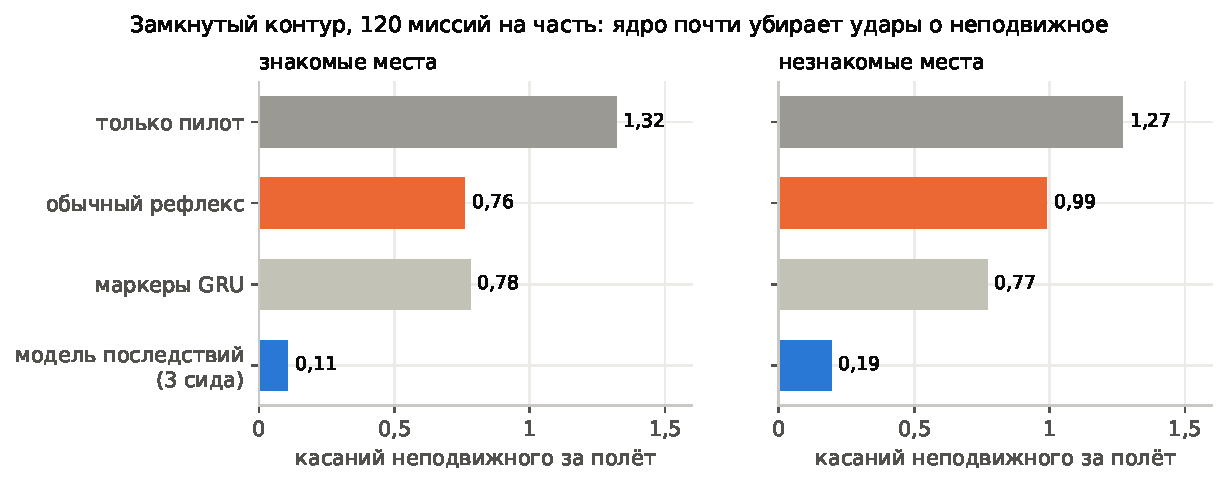
\includegraphics[width=\linewidth]{fig_closed_loop_ru.pdf}
\caption{Замкнутый контур, 120 миссий на часть, одни и те же миссии для всех быстрых слоёв. Касаний неподвижного за 40-секундный
полёт. Ядро с соматическими маркерами (синее, среднее трёх сидов) почти убирает удары о неподвижное в знакомых и незнакомых местах.}
\label{fig:closed}
\end{figure}

\paragraph{Замкнутый контур.} На одних и тех же 120 миссиях на часть (рис.~\ref{fig:closed}) ядро снижает удары о неподвижное на
92\,\% в знакомых и 85\,\% в незнакомых местах, все касания на 67 и 54\,\% (среднее трёх сидов). Против обычного рефлекса на тех же
миссиях это $-0{,}77$\ci{-1{,}06}{-0{,}50} и $-0{,}77$\ci{-1{,}07}{-0{,}49} касания на полёт. Ядро обучено на данных пилота,
который из-за найденной позже ошибки висел после первой паузы, а летает с исправленным: перенос на другое поведение сработал.
За это дрон теряет от 12 до 13\,\% хода миссии за 40\,с. Попадания встреч почти не меняются, большинство из них физически неизбежны.

\section{Медленные решения: решает ядро, БЯМ не добавляет}\label{sec:slow}
В пять моментов 120-секундного полёта (около 12, 30, 48, 66 и 84\,с, каждый со сдвигом до 2\,с) дрон выбирает: продолжать, подняться и продолжать, ждать 10\,с, сесть сейчас или домой.
Лучший вариант определяет раздвоение мира (раздел~\ref{sec:method}). Мы дообучили Qwen2.5-1.5B \citep{qwen25} с LoRA \citep{hu2022lora} (ранг 16, $\alpha=32$, прореживание 0,05 на всех
проекциях внимания и MLP; AdamW с шагом $2\cdot10^{-4}$, 8 эпох для каждого варианта) на семи вариантах входа, по три сида, с
перемешанным порядком ответов (рис.~\ref{fig:llm}). В каждом запросе есть время в воздухе, число оставшихся участков, оставшийся
путь и расстояние до дома. Вариант N больше ничего не добавляет; T добавляет сырую телеметрию словами (спутники GPS и HDOP, время
и путь без хорошей отметки, источник скорости, заряд, высота, скорость, ветер); F добавляет семь чувств в процентах; FT~--- и то
и другое. В вариантах со слотами логиты чувств (Fs) или одиннадцать чисел телеметрии (Ts) проходят через небольшую сеть
(64 нейрона GELU) в четыре входных вложения БЯМ, которые обучаются с шагом $10^{-3}$; FsT соединяет слоты чувств с телеметрией
словами.
\begin{figure}[t]
\centering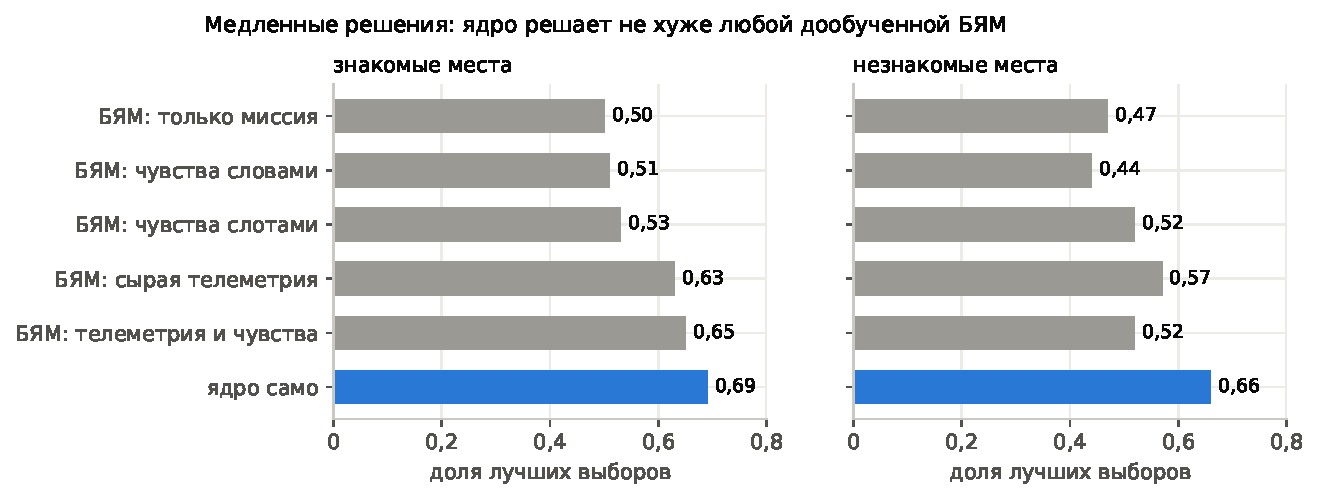
\includegraphics[width=\linewidth]{fig_llm_decisions_ru.pdf}
\caption{Медленные решения: доля лучших выборов (среднее трёх сидов). Ядро само (маленькая политика на чувствах и телеметрии)
решает не хуже любой дообученной БЯМ. Чувства словами не лучше сырой телеметрии.}
\label{fig:llm}
\end{figure}
Чувства словами не обошли сырую телеметрию (разница $+0{,}02$\ci{-0{,}03}{0{,}07} в знакомых и $-0{,}05$\ci{-0{,}11}{0{,}01}
в незнакомых местах). Чувства мягкими слотами в пространстве вложений обошли те же чувства словами в незнакомых местах
($+0{,}08$\ci{0{,}03}{0{,}13}), и модели со слотами опирались на чувство «мало сил»: если его перевернуть, они теряли от 0,10 до 0,12.
Передача БЯМ решений, в которых ядро меньше всего уверено, только вредила (0,69 падает до 0,63, если отдать все). Сообщения словами
о будущем мира (фронт ветра, глушение GPS, холод; 25\,\% ложных) модель не читала: если убрать их из обученной модели, ничего не
меняется ($0{,}00$\ci{-0{,}01}{0{,}01}). БЯМ, получившая суждение ядра о каждом варианте, сильно ему доверяла (подмена суждения
стоила от 0,16 до 0,26), и все шесть таких моделей обучились устойчиво, а на сырых числах четыре модели из шести свелись к одному
ответу. Третий этап с сильными событиями остановило правило пилота: объявленное событие меняло лучший план лишь в 15\,\% решений
при пороге 20\,\%. Проверка заняла десять минут процессора вместо часов обучения на видеокарте.

\section{Кто выбирает цель: модель зрения и языка против геометрии}\label{sec:vlm}
В 400 сценах с похожими объектами (в 70\,\% есть близнец того же вида и цвета) Qwen2.5-VL-7B \citep{qwen25vl} без дообучения
обвела описанную цель в 0,19 трудных видимых сцен. Это ниже выбора «ближайший к примерной точке» (0,38) и угадывания (0,34). С
номерами объектов \citep{yang2023som} вышло от 0,41 до 0,46, с видами крупно каждого кандидата 0,50\ci{0{,}42}{0{,}58}. Кодировщик предложений с идеальным
восприятием дал 0,69 на новых формулировках. Новые слова модели не мешали, а вот близнецов по размеру и отношениям она не
различала. Правила, записанные заранее, не выполнены, и контур с такой моделью не строился.

\section{Целые миссии по одному запросу в настоящих местах}\label{sec:missions}
\paragraph{Система.} Текст оператора превращает в структуру миссии Qwen2.5-1.5B с LoRA (те же настройки LoRA, две эпохи), обученная на шаблонах и 4591 перефразе от
Qwen2.5-7B с обратной проверкой смысла. Она точна на 56\,\% из 100 рукописных русских заданий (порог 85\,\%), поэтому оператор
подтверждает разбор в приложении. Детектор YOLO11s \citep{yolo11}, обученный на размеченных кадрах обучающих мест, на местах
проверки находит 0,974 объектов при точности 0,978 (цвет 0,958). Выбор цели геометрический: отношения считаются по карте и
найденным объектам, описания построены по \citet{dale1995}. Навигация объединяет счисление, лидарно-инерциальную одометрию и
фильтр частиц «лидар против карты» (без GPS ошибка от 0,25 до 0,8\,м на маршруте 1,2\,км на высоте от 25 до 30\,м). Конечный автомат
летит над крышами по карте, ищет, подлетает ближе, перед касанием проверяет вблизи все названные признаки, действует и
возвращается. Касающиеся действия (посадка, сброс, захват, влёт) дрон выполняет сам только для \emph{однозначной} цели, иначе
спрашивает оператора или пропускает шаг.

\paragraph{F4 и F5 (500 миссий на местах проверки; отказ GPS назначен в 187 и успел случиться до конца миссии в 175, атаки птиц в 256, ветер с порывами).} Первый прогон по
заранее записанному плану не выполнил правило безопасности (ошибка цели 3,2\,\% при пороге 2\,\%). После правила однозначной цели
и исправлений, найденных по трассам полётов, ошибка цели упала до 1,6\,\%, а затем до 0,67\,\%\ci{0}{1{,}67}
(точная верхняя граница Клоппера--Пирсона 2,4\,\%; таблица~\ref{tab:f4}). Без ядра (обычный рефлекс вместо соматических маркеров) миссий с касанием неподвижного стало 11,0\,\% против
5,4\,\%, это $-0{,}28$\ci{-0{,}48}{-0{,}11} касания на миссию, а в 173 миссиях, где GPS пропал в обоих прогонах, 0,77 против 0,25 на миссию. Сырая телеметрия вместо
медленных чувств разницы не дала, но эти чувства в коротких миссиях почти не срабатывали («потерялся» в 23 миссиях из 500, «мало
сил» в двух). Раздел~\ref{sec:stageg} проверяет их там, где они должны быть нужны.

\begin{table}[t]
\centering\small
\caption{Целые миссии в незнакомых местах. F4~--- первый прогон по плану; F4b и F4d исправляют ту же систему после него и
приводятся как исправления. В скобках 95\,\% бутстрэп-интервалы по миссиям. Правило F4 ограничивает саму долю, правило
этапа G~--- верхнюю границу её интервала.}
\label{tab:f4}
\begin{tabular}{@{}lccc@{}}
\toprule
 & F4 (500) & F4b (500) & F4d (300) \\
\midrule
Выполнено шагов & 0,289 & 0,266 & 0,322 \\
Ошибка цели (правило до 2\,\%) & 3,2\,\%\ci{1{,}8}{4{,}8} & 1,6\,\%\ci{0{,}6}{2{,}8} & 0,67\,\%\ci{0}{1{,}67} \\
Миссий с касанием неподвижного & 5,0\,\% & 5,4\,\% & 3,3\,\% \\
\bottomrule
\end{tabular}
\end{table}

\section{Итоговая проверка и повреждения на новых миссиях}\label{sec:stageg}
Все части этого этапа вместе с порогами записаны до прогонов (этап G). Места проверки те же, кварталы Токио и Казани, но 300
миссий новые: новые расстановки, тексты, примерные точки и отказы. Ничего в системе на них не настраивалось.

\paragraph{Итоговая проверка (G2).} В таблице~\ref{tab:g2} система работает одна (текст оператора разбирает модель F3b, на
вопросы дрона никто не отвечает), а рядом та же система с обычным рефлексом вместо ядра чувств, на тех же 300 миссиях. Главный
результат проекта повторился на новом наборе и стал сильнее: без ядра касаются неподвижного 14,7\,\% миссий, с ядром 4,3\,\%
(парная разница $-10{,}3$ процентного пункта\ci{-14{,}7}{-6{,}0}; $-0{,}61$\ci{-0{,}92}{-0{,}35} касания на миссию). Впервые
ядро снизило и попадания атакующих птиц ($-0{,}19$\ci{-0{,}33}{-0{,}06} на миссию с атакой), а система с ядром выполнила больше
шагов ($+0{,}038$\ci{0{,}008}{0{,}070}). Правило безопасности, записанное заранее, не выполнено: без помощи оператора дрон коснулся не
той цели в 3 миссиях из 300, это 1,0\,\% с верхней бутстрэп-границей 2,3\,\% (точная граница Клоппера--Пирсона 2,9\,\%) при требуемых 2\,\%. Рис.~\ref{fig:lesion} ставит это повторение рядом
с первым опытом с повреждением.

\begin{table}[t]
\centering\small
\caption{Итоговая проверка на 300 новых миссиях в незнакомых местах (G2). Миссии одни и те же для обоих вариантов; в скобках
95\,\% бутстрэп-интервалы по миссиям. Разница парная.}
\label{tab:g2}
\setlength{\tabcolsep}{3.5pt}
\begin{tabular}{@{}lccc@{}}
\toprule
 & Ядро чувств (один) & Обычный рефлекс & Разница \\
\midrule
Миссий с касанием неподвижного & \textbf{4,3\,\%}\ci{2{,}3}{6{,}7} & 14,7\,\%\ci{10{,}7}{18{,}7} & $-10{,}3$\ci{-14{,}7}{-6{,}0}\,п.п. \\
Касаний неподвижного на миссию & & & $-0{,}61$\ci{-0{,}92}{-0{,}35} \\
Попаданий на миссию с атакой & & & $-0{,}19$\ci{-0{,}33}{-0{,}06} \\
Выполнено шагов & 0,301\ci{0{,}254}{0{,}348} & 0,257\ci{0{,}214}{0{,}304} & $+0{,}038$\ci{0{,}008}{0{,}070} \\
Выполнено миссий целиком & 0,287\ci{0{,}233}{0{,}340} & 0,253\ci{0{,}207}{0{,}303} & $+0{,}033$\ci{0{,}003}{0{,}063} \\
Не та цель (правило до 2\,\%) & 1,0\,\%\ci{0}{2{,}3} & 2,3\,\%\ci{0{,}7}{4{,}0} & $-1{,}3$\ci{-3{,}0}{-0{,}3}\,п.п. \\
\bottomrule
\end{tabular}
\end{table}

\begin{figure}[t]
\centering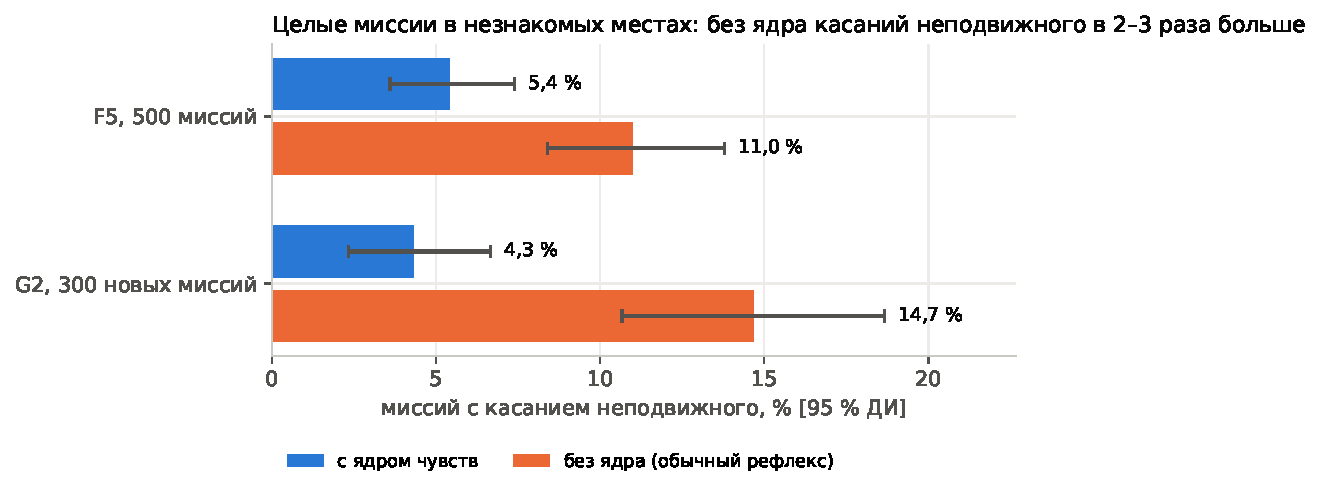
\includegraphics[width=.92\linewidth]{fig_missions_lesion_ru.pdf}
\caption{Целые миссии в незнакомых настоящих местах с ядром чувств и с обычным рефлексом вместо него. F5~--- первый опыт с
повреждением (500 миссий), G2~--- 300 новых миссий. Интервалы: 95\,\% бутстрэп по миссиям.}
\label{fig:lesion}
\end{figure}

\paragraph{Один и с оператором.} По действиям дрон в одиночку выполнил пролёт в 0,49 шагов, посадку в 0,44, осмотр в 0,30,
захват крюком в 0,29, сброс на парашюте в 0,22 и влёт в ангар в 0,14. Большая часть неудач~--- это отказы по замыслу: если описание
не выделяет один объект, дрон не трогает ни один. Приложение задумано для работы с человеком, который проверяет разбор и отвечает
на вопросы дрона, поэтому первые 200 миссий мы пролетели ещё раз именно так. Оператор в симуляции получает верный разбор и на
вопрос выбирает того кандидата, который стоит у задуманного объекта. На 182 миссиях, закончившихся до предела времени прогона
(18 ещё летели), дрон с оператором выполнил 0,56 шагов против 0,29 в одиночку на тех же миссиях (парная разница
$+0{,}27$\ci{0{,}20}{0{,}33}) и 0,54 миссий целиком против 0,29 (рис.~\ref{fig:actions}). Большинству миссий вопрос вообще не
понадобился (медиана 0, 90-й процентиль 1). У помощи есть цена: теперь дрон долетает каждый шаг до конца, и миссий с касанием
неподвижного стало 10,4\,\% вместо 3,8\,\% ($+6{,}6$\ci{2{,}7}{10{,}4} п.п.). Не той цели он коснулся в 4 миссиях (2,2\,\%), две
из них~--- это те же ошибки, что и в одиночку, без вопроса. В трёх миссиях, где ни один кандидат не был целью, дрон спрашивал снова и
снова (от 131 до 541 раза), и приложению там нужен предел.

\begin{figure}[t]
\centering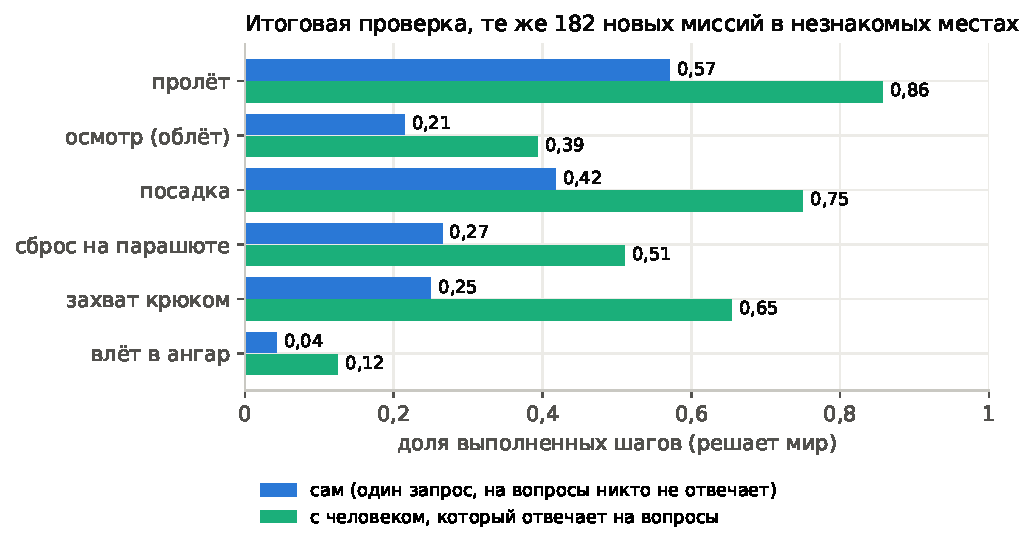
\includegraphics[width=.8\linewidth]{fig_actions_ru.pdf}
\caption{Выполненные шаги по действиям на тех же 182 новых миссиях: дрон один и дрон с человеком, который проверяет разбор и
отвечает на вопросы. Засчёт по миру: на что сел, куда упал груз, что висит на крюке.}
\label{fig:actions}
\end{figure}

\paragraph{Дверь ангара (G1).} Влёт в ангар был самым слабым действием, и одна разобранная неудача показала, что искатель двери
принял щель в задней стене за дверь. Мы попробовали правило строже: проём считается, только если сквозь него лидар видит пол
ангара. Когда дрон ставили на окружность вокруг 90 ангаров, старый искатель нашёл верную дверь у 74 из 76 открытых ангаров и ни
одной двери у 14 закрытых; новый нашёл 72, пропустил 4 и увидел дверь у 3 закрытых. В полёте, с верным разбором и человеком,
который отвечает на вопросы дрона, новый искатель влетел в 1 ангар из 38 полётов, старый в 6 из 37. Пока дрон облетает ангар,
его собственная оценка положения уплывает и размазывает точки стен по коробке. По правилу, записанному заранее, остаётся старый
искатель.

\paragraph{Медленные чувства в тяжёлых миссиях (G3).} Медленные чувства («я потерялся», «мало сил») в коротких миссиях F5 почти
не срабатывали, поэтому этап G проверил их там, где они должны быть нужны. В 120 тяжёлых миссиях на местах проверки заряд при
взлёте от 30 до 65\,\%, в 60\,\% миссий батарея холодная, ветер от 3 до 9\,м/с, GPS пропадает (в 47 из 99 пролетевших миссий) или подменяется (в 26), есть атаки птиц,
и возврат домой обязателен. Разбор верный, так что проверяется только медленный слой. Пять вариантов летели одни и те же миссии:
чувства ядра; сырая телеметрия с порогами вместо них, которая сравнивает заряд с энергией на дорогу домой; без медленного слоя; и
без каждого чувства по очереди. Из-за предела времени успели 99 миссий (98 у трёх вариантов; рис.~\ref{fig:slow}).

С чувствами ядра батарея села в воздухе в 29\,\% миссий, без медленного слоя тоже в 29\,\% (парная разница
$0{,}0$\ci{-7{,}1}{7{,}1} п.п.). Первое ожидание, что медленный слой предотвращает такие падения, не подтвердилось. Сырая
телеметрия справилась лучше: 16\,\% падений ($-13{,}1$\ci{-21{,}2}{-5{,}1} п.п. против чувств) и больше посадок дома (63 против
52\,\%, $+11{,}1$\ci{5{,}1}{18{,}2}). Заплатила она меньшим числом целых миссий ($-0{,}040$\ci{-0{,}081}{-0{,}010}), потому что
вдвое чаще поворачивала домой раньше времени. Значит, H6 не подтверждена, как мы и записали заранее: чувство «мало сил» обучено
на 40-секундных эпизодах и не знает расстояния до дома, а правило телеметрии умножает расход на это расстояние. Чувство
действовало (с ним дрон раньше времени поворачивал домой в 13\,\% миссий, без него ни разу), но падений меньше не стало
($0{,}0$\ci{-6{,}1}{6{,}1}). Без «я потерялся» не изменились ни падения, ни возвраты. Одно наблюдение не планировалось: без
«я потерялся» дрон реже касался неподвижного ($-0{,}22$\ci{-0{,}43}{-0{,}06} касания на миссию). Для настоящего аппарата вывод
простой. Запас энергии должно считать явное правило по расстоянию и расходу, а не выученное чувство.

\begin{figure}[t]
\centering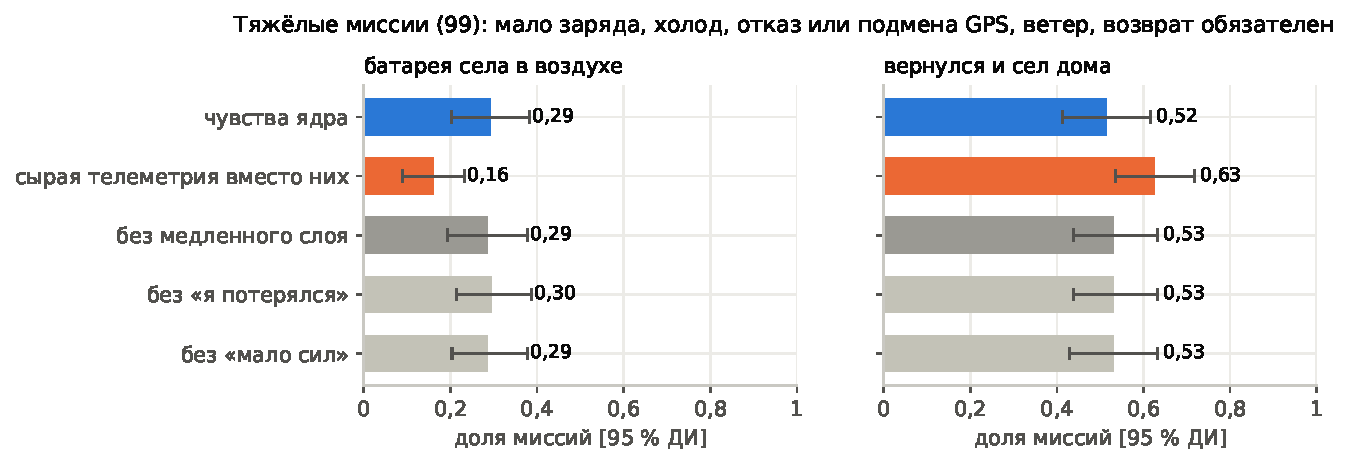
\includegraphics[width=\linewidth]{fig_slow_ru.pdf}
\caption{Тяжёлые миссии (G3), одни и те же для всех вариантов. Слева миссии, где батарея села в воздухе, справа миссии, которые
кончились посадкой дома. Сырая телеметрия с правилом «энергия до дома» лучше выученных медленных чувств; без медленного слоя или
без одного чувства ничего не меняется. Интервалы: 95\,\% бутстрэп по миссиям.}
\label{fig:slow}
\end{figure}

\paragraph{Ложные и запоздавшие чувства (G4).} Пациенты Дамасио подсказывают ещё два повреждения: чувство, которое срабатывает,
когда ничего нет, и чувство, которое приходит слишком поздно. На первых 100 миссиях итоговой проверки мы ещё дважды пролетели
полную систему. В первом варианте маркер «продолжать» показывал опасность в пустом небе на 1\,с в случайные моменты, примерно раз
в 20\,с; во втором маркеры видели мир на 0,3\,с позже. Ложные тревоги добавили 24 перехвата на миссию\ci{19}{29} и не стоили
шагов ($+0{,}015$\ci{-0{,}05}{0{,}08}), но миссий с касанием неподвижного стало 9\,\% вместо 4\,\% ($+5{,}0$\ci{0{,}0}{10{,}0}
п.п.). Лишний отворот на улице сам может кончиться стеной. Мы ждали меньше шагов и не меньше касаний; вторая половина ожидания
сбылась, первая нет. Запоздание на 0,3\,с почти ничего не изменило: миссий с касанием неподвижного $+3{,}0$\ci{-1{,}0}{8{,}1}
п.п., так что ожидаемый рост не подтвердился. Маркеры смотрят на 2\,с вперёд, и задержка в 0,3\,с мала против этого горизонта.

\subsection{К настоящему аппарату: мозг на автопилоте PX4}\label{sec:px4}
Дрон летает на автопилоте, а не на регуляторе нашего симулятора. Мы написали мост MAVLink, который даёт неизменённому мозгу миссии
тот же интерфейс на настоящем автопилоте (PX4 \citep{meier2015px4} или ArduPilot): телеметрия на вход, заданные скорости на выход с частотой 20\,Гц,
перевод систем координат, сторожевой таймер, который держит точку, если мозг опаздывает, и собственные защиты автопилота под всем
этим. Затем мы провели 12 миссий (посадка, сброс, захват, осмотр, пролёт, цели на земле) на программной сборке PX4 с её моделью
квадрокоптера SIH, каждые 0,1\,с ставя наш мир в оценённое PX4 положение, чтобы лидар, камера и засчёт оставались нашими. Мост
сработал механически: PX4 включал моторы, взлетал, выполнял команды мозга, садился, снова включался и отказывался взлетать, когда
отказывали его датчики. Успех миссий не перенёсся: 1 из 12 миссий с PX4 против 7 из 12 с нашим регулятором на тех же миссиях, и
удержание точки собственным контуром положения PX4 в точных фазах ничего не изменило. PX4 отрабатывает команды скорости мозга с
медианной ошибкой от 0,8 до 1,3\,м/с, и миссии шли примерно вдвое дольше. Тайм-ауты, скорости и точные фазы мозга настроены на нашем
регуляторе; до любого полёта их нужно перенастроить и заново проверить на настоящем автопилоте.


\section{Обсуждение}
\paragraph{Для чего хороши чувства.} Ядро сжимает тысячи раздвоенных последствий в откалиброванное «продолжу и во что-то врежусь»
и оценивает каждое возможное действие по его эфферентной копии. Получается сильный быстрый регулятор. Его выигрыш держится в
незнакомых местах, при другом пилоте, на трёх сидах, в целых миссиях с восприятием и языком в контуре и на новом наборе миссий.
Это самый ясный положительный результат проекта и машинный аналог проверки Дамасио: если убрать ядро и оставить все сырые данные
и обычный рефлекс, миссий с касанием неподвижного становится в 2,0 (F5) и 3,4 раза (G2) больше.
\paragraph{Где БЯМ помогает.} В наших задачах БЯМ пригодилась один раз, чтобы превратить свободный запрос в структуру миссии.
Решения, которые определяют числа, быстрые или медленные, маленькое ядро принимает не хуже. БЯМ с суждением ядра ему доверяют и
учатся устойчиво, но пользы не добавляют. Слова о будущем мира модели игнорировали, а 7B-модель зрения не нашла описанный объект
среди близнецов. Мы видим здесь границу: язык нужен там, где на языке задана \emph{цель}.
\paragraph{Методические уроки.} Исследователь не должен задавать ни чувство, ни ответ. Дешёвый пилот с раздвоением мира
показывает, \emph{может} ли БЯМ вообще повлиять, ещё до дорогого обучения. Многие ранние «результаты» оказались ошибками: трекер
с 99,6\,\% мусорных треков, пилот, который висел после первой паузы, засчёт, не видевший пола ангара, автопилот без интегратора по
горизонтали, застревавший в метре от точки при ветре 7\,м/с, петля из 613 вопросов оператору. Каждую нашли, читая трассы полётов,
а не средние числа.

\section{Ограничения}
Все результаты получены в симуляции (MuJoCo, синтетические кадры); зрение обучено на синтетике, для настоящих камер его нужно
дообучить на настоящих снимках. Медленные чувства обучены на 40-секундных эпизодах и не знают расстояния до дома, в тяжёлых миссиях
правило по телеметрии оказалось лучше них (раздел~\ref{sec:stageg}). Маленькие птицы
остаются пределом датчика. Второй симулятор планировался, но не сделан. Модель разбора текста ниже своих порогов. Из-за бюджета
часть прогонов меньше запланированных. Проверка с PX4 сводит прошивку автопилота с нашим миром и показывает, что мозг миссии,
настроенный на наш регулятор, без перенастройки теряет на PX4 большую часть успеха (раздел~\ref{sec:px4}). Проверки целых миссий
включали отказ и подмену GPS, ветер и атаки птиц; отказов лидара, тумана и сбитого компаса в них не было. Ручной полёт в приложении
с постоянными ложными точками лидара, подменой GPS и туманом показал изъян мозга миссии. Он набирал высоту каждый раз, когда лидар
видел впереди то, чего нет на карте, не отсеивая шум и без потолка высоты. Высоко над крышами лидар терял стены, а с ними и
сопоставление с картой, которое ловит подмену GPS. В выложенном приложении одиночные точки лидара отбрасываются, высота набирается
только при препятствии, видном три скана подряд, и не выше 120\,м; описанные проверки шли без этих исправлений.

\section{Заключение}
Ядро чувств, выращенное только на последствиях, даёт дрону быстрые откалиброванные соматические маркеры. В незнакомых местах они
в 2,0 и 3,4 раза (F5 и G2) снижают число миссий с касанием зданий, а в проверке быстрой реакции почти убирают удары. В наших задачах
языковая модель нужна для языка, то есть для запроса оператора, а не для решений, которые чувства уже принимают хорошо.
\GCONCL

\section*{Этика и последствия}
Работа ограничена гражданскими задачами: каждая цель, которую знают модель разбора и детектор,~--- место или сооружение
(посадочная площадка, крыша, ангар, площадка для сброса), никогда не человек и не машина. Автономные дроны можно использовать во
вред, поэтому мы прямо пишем, чего системе ещё не хватает для настоящего полёта (раздел~\ref{sec:px4}). Настоящие полёты должны
идти по воздушному законодательству, с оператором, который может взять управление. В предварительном исследовании использовались
только открытые наборы данных (CREMA-D, ESConv, PRISM) по их лицензиям; новых данных от людей не собиралось.

\section*{Благодарности}
Благодарим участников Open\-Street\-Map и разработчиков MuJoCo, PX4, Qwen и Ultra\-lytics. Часть кода и текста подготовлена с помощью
ассистента на основе ИИ (Claude, Anthropic); замысел исследования, решения и проверка всех результатов принадлежат автору.

\section*{Код, данные и видео}
Код, планы миссий, журналы полётов, обученные модели и скрипты анализа приложены к статье как дополнительные материалы,
вместе с планом каждого этапа, его гипотезами и порогами, записанными до прогонов. Дополнительные видео повторяют десять миссий
итоговой проверки (G2) со всеми системами на экране, они охватывают все шесть действий; четыре из них показаны ещё раз с обычным
рефлексом вместо ядра чувств. Ещё четыре видео повторяют эти миссии с обоими дронами рядом в одном кадре (рис.~\ref{fig:compare}),
а одно показывает задание в приложении от начала до конца (рис.~\ref{fig:app}). Лицензии: код выпускается под AGPL-3.0, потому что вызывает Ultralytics YOLO11; модели и данные~---
под CC BY 4.0, кроме детектора (AGPL-3.0); данные карт \copyright{} участники OpenStreetMap, ODbL.

{\small
\bibliographystyle{plainnat}
\bibliography{refs}
}

\appendix
\section{Постоянные правила (кратко)}
Чувства и ответы берутся только из данных людей или физики мира. До обучения дешёвая проверка на процессоре показывает, что
сигнал несёт что-то сверх слов. Гипотезы и пороги записываются до прогона. Сидов два-три и больше. Настройка идёт только на
обучающих данных. Считаются события, а не шаги симуляции. Всё случайно (скорости до 1000\,м/с, направления, отказы с настоящими
причинами), есть ловушки и генератор встреч, чтобы угрозы действительно встречали дрон. Проверка идёт на незнакомых семействах и
местах, неизбежные события показываются отдельно. Каждый кирпич восприятия сверяется с истиной симулятора. Сиды устойчивые
(CRC32). Дообученная модель должна обходить лучший постоянный ответ. Сравниваемые условия получают одинаковое число эпох.
Применение только гражданское: цели~--- это места и сооружения, никогда не люди и не машины.

\section{Вычисления}
Все тяжёлые прогоны шли на облачных машинах с одной видеокартой (RTX 3080, 3090 или 4090). На борту
ядро работает в NumPy быстрее миллисекунды на шаг, детектор~--- YOLO11s.

\section{Видео к статье}
Каждое видео~--- это повтор записанного полёта на местах проверки; файлы и список того, что происходит в каждом, приложены к статье.
На рис.~\ref{fig:frame} кадр из видео миссии, на рис.~\ref{fig:compare} кадр видео «рядом», на рис.~\ref{fig:app}
приложение в полёте.

\begin{figure}[h]
\centering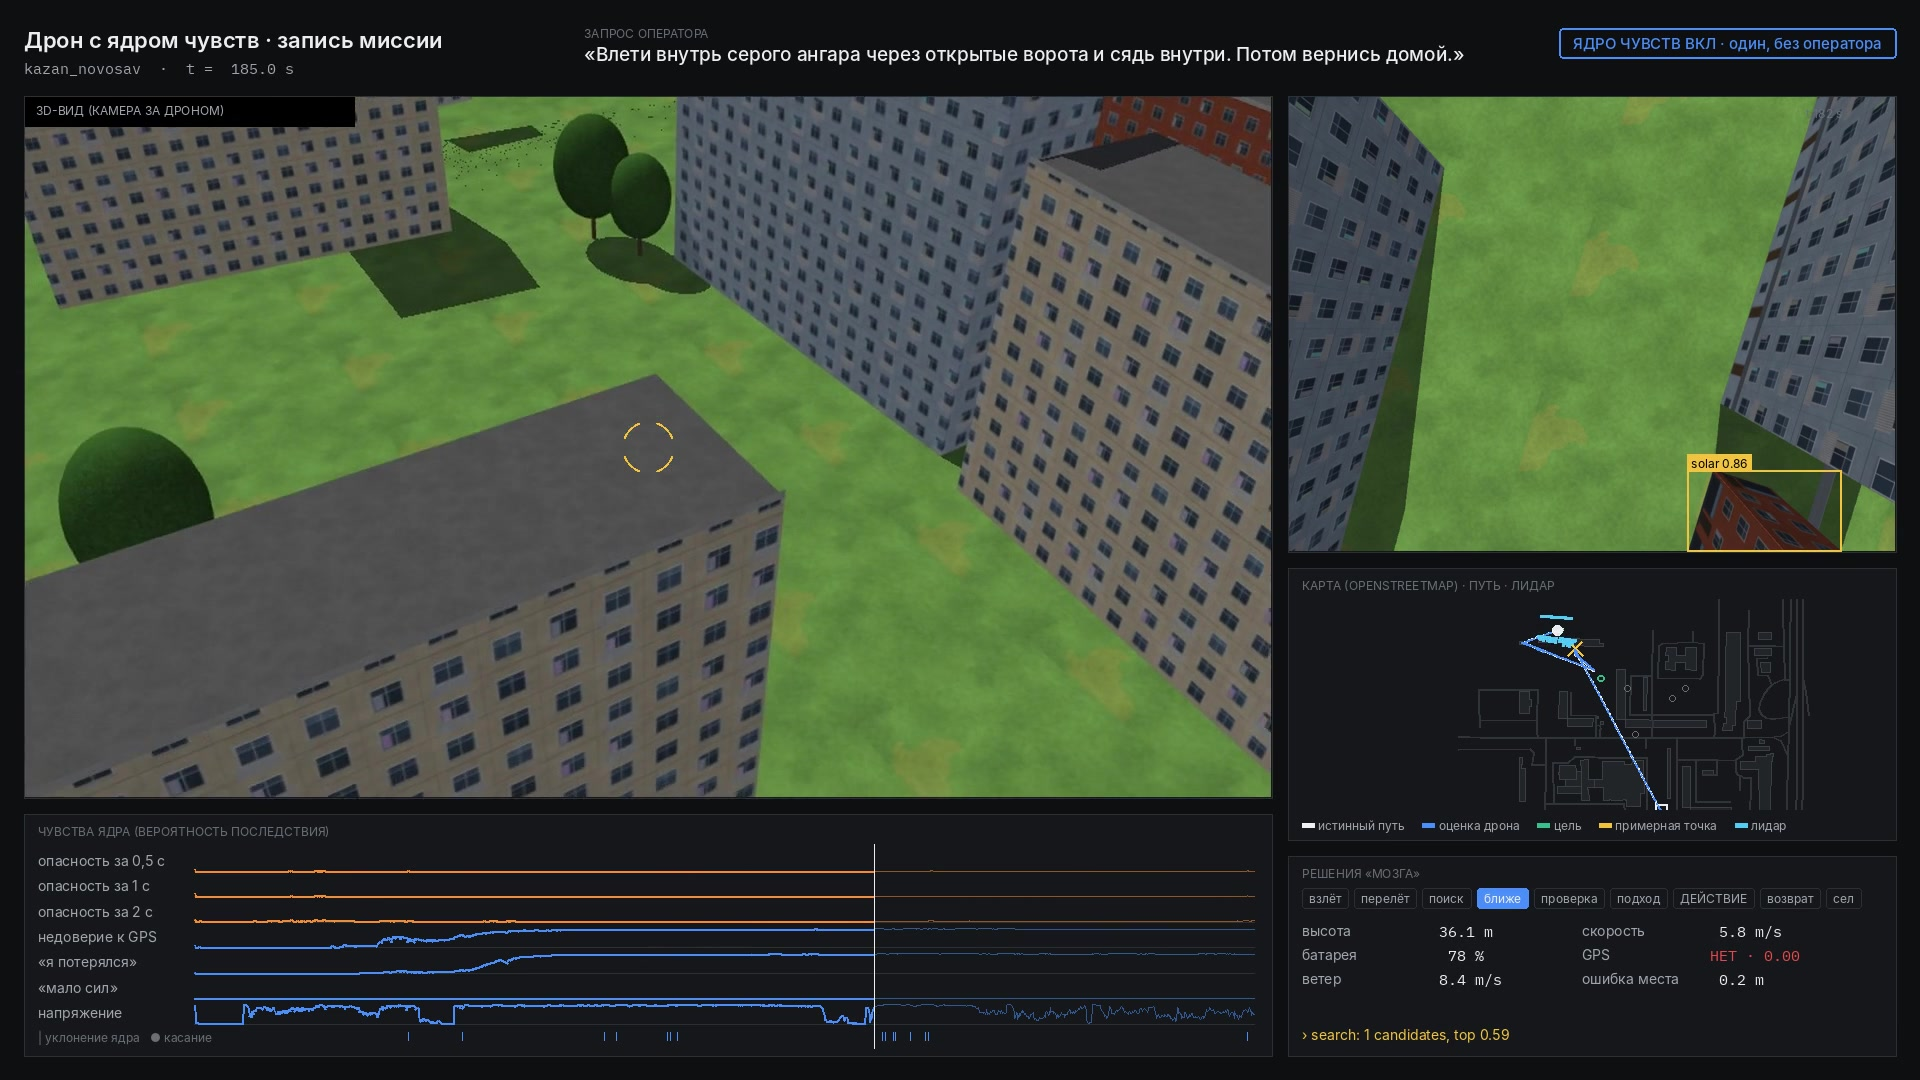
\includegraphics[width=\linewidth]{frame_mission_ru.jpg}
\caption{Кадр миссии G45 (влететь в серый ангар и вернуться домой) в казанском районе проверки, 185\,с полёта. GPS пропал на
36\,с, дрон летит по лидару и карте, и его чувство «я потерялся» выросло. Слева вид сзади и чувства ядра за весь полёт с
моментами, когда оно перехватывало команду мозга. Справа камера дрона с найденными объектами, карта с истинным путём, собственной
оценкой дрона и примерной точкой, а ниже этап и состояние мозга миссии.}
\label{fig:frame}
\end{figure}

\begin{figure}[h]
\centering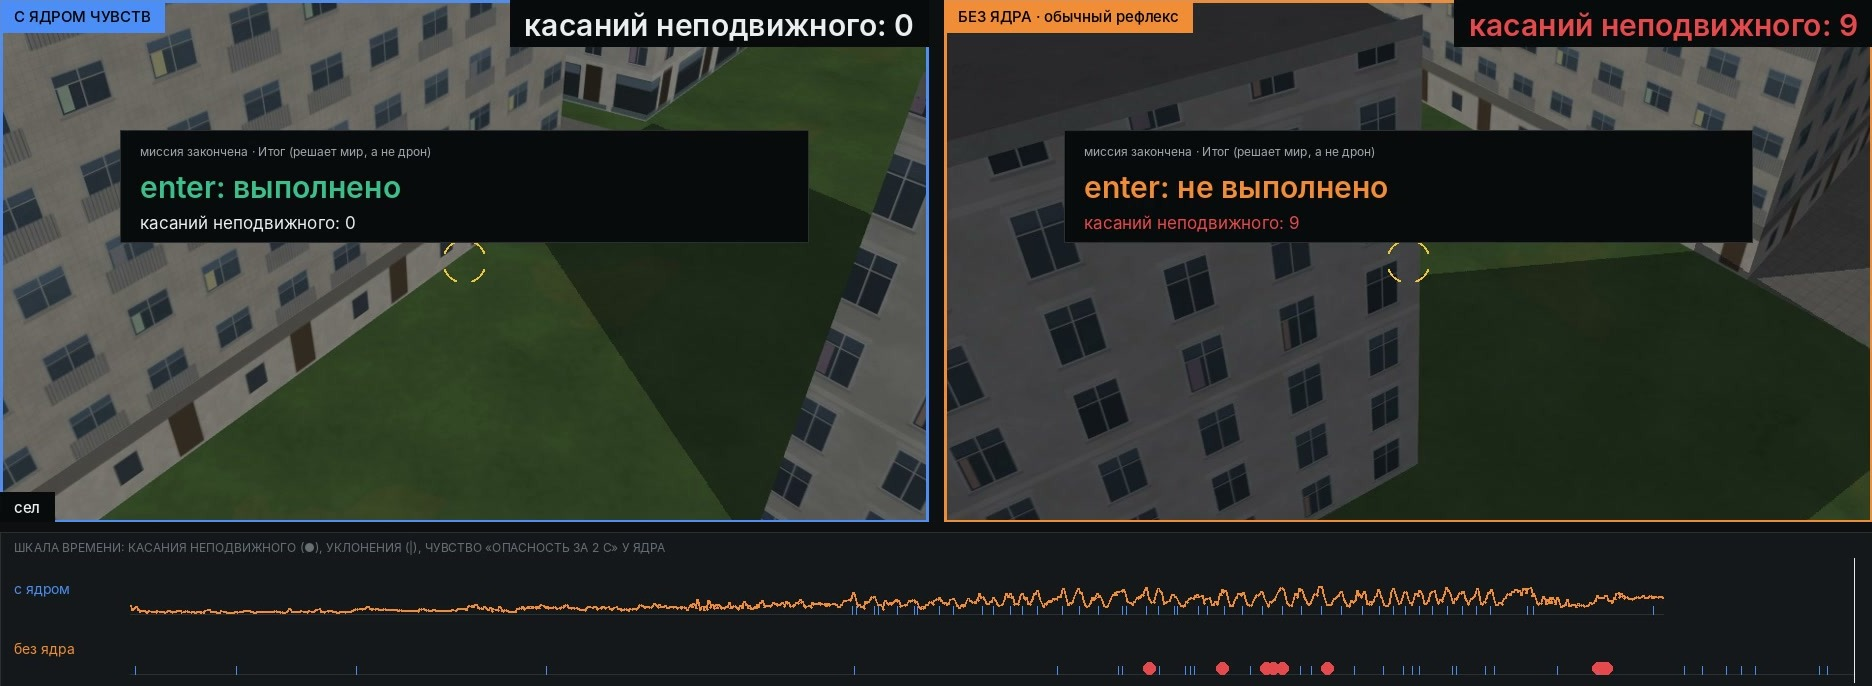
\includegraphics[width=\linewidth]{fig_compare_ru.jpg}
\caption{Кадр видео «рядом» для миссии G206 (влететь в синий ангар, токийский район проверки): одна и та же миссия с ядром чувств
(слева) и с обычным рефлексом вместо него (справа), в конце миссии. С ядром дрон влетел в ангар, ничего не задев; с рефлексом влёт
не удался после 9 касаний неподвижного. Внизу шкала всего полёта: касания неподвижного у каждого дрона (красные точки) и чувство
ядра «опасность за 2\,с». Четыре видео «рядом»~--- это повторы миссий G2 по их
планам на другой модели видеокарты; малые численные различия детектора меняют ход полёта, поэтому повтор в деталях отличается от
записанного полёта G2. На четырёх повторах у ядра 1 касание неподвижного, у рефлекса 16; в одном из них (G112) разницы нет, а в
другом (G45) ядро не выполнило влёт в ангар, который рефлекс сделал ценой 6 касаний.}
\label{fig:compare}
\end{figure}

\begin{figure}[h]
\centering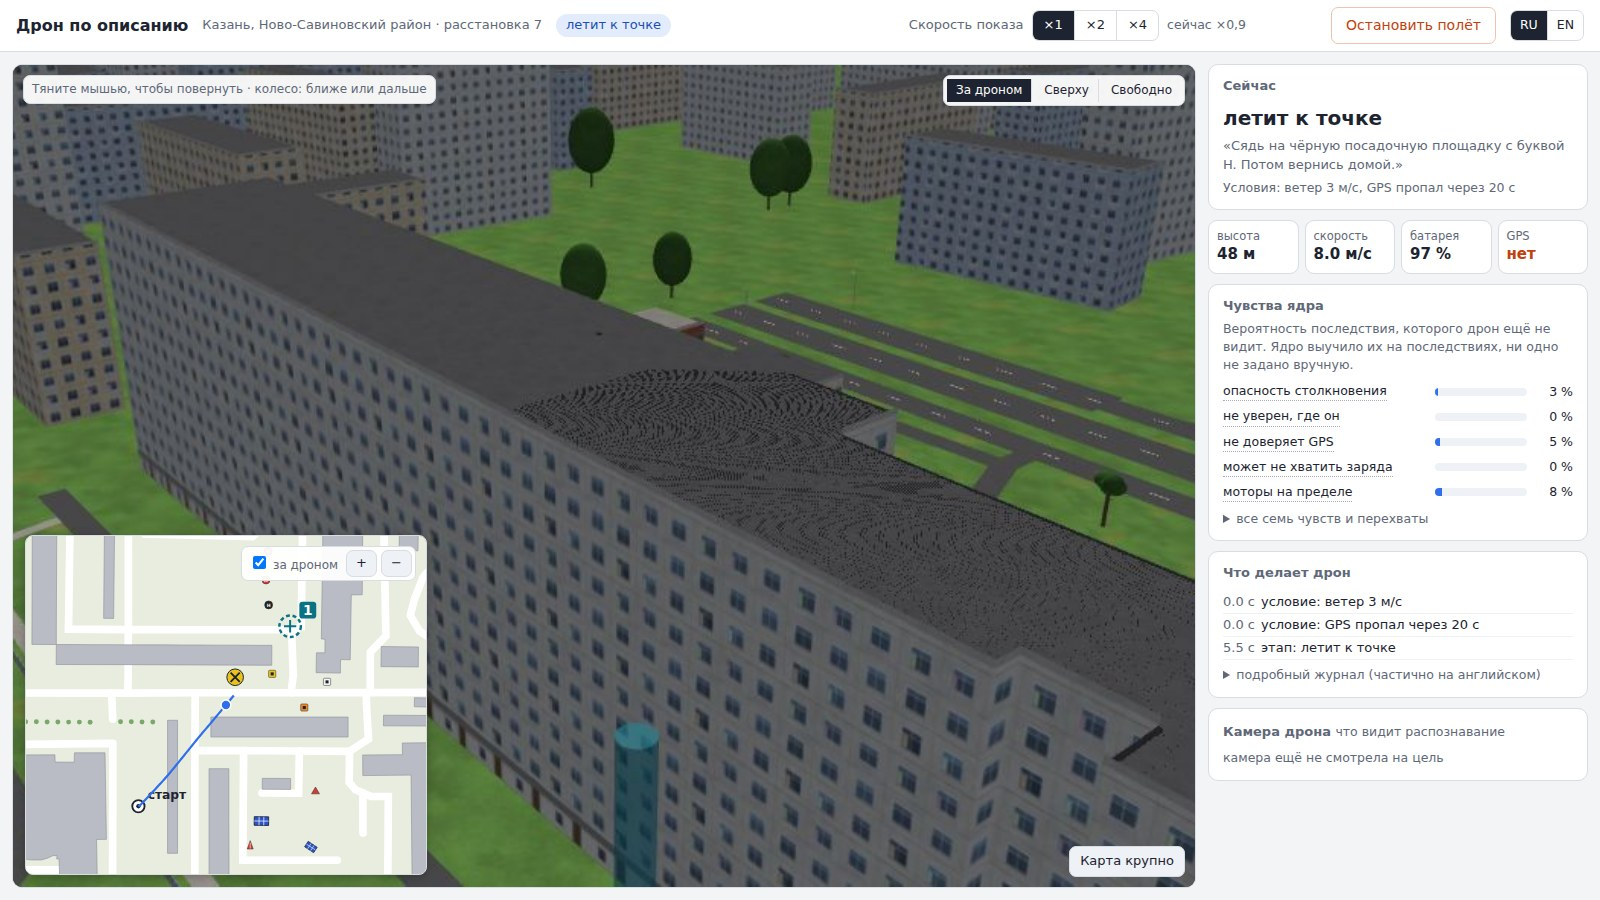
\includegraphics[width=\linewidth]{fig_app_ru.jpg}
\caption{Приложение в полёте. Крупный 3D-вид за дроном рисует сам симулятор; карта в углу показывает примерную точку, истинный путь
и собственную оценку дрона. Справа этап полёта, условия (здесь GPS пропал через 20\,с), высота, скорость, батарея и GPS, пять
чувств ядра и лента событий. До полёта оператор ставит примерную точку, пишет задание, проверяет разбор, показанный простыми
словами, и выбирает условия.}
\label{fig:app}
\end{figure}


\end{document}
